% set 0.5 inch indentation
\setlength{\parindent}{0in}
% set paragraph space = 0 space
\setlength{\parskip}{1.5mm}
% set line space 1.5
\setlength{\baselineskip}{1.6em}

\chapter{INTRODUCTION}
\section{Background}
\acrfull{vl} models have gained significant attention due to their ability to perform both zero-shot and transfer learning, achieving high performance across numerous downstream tasks through pre-training with web-scale image-text pairs \cite{s-clip, medclip, vl-review}.
Many \acrshort{vl} models incorporate \acrfull{mlm} as a pre-training task, making it a fundamental approach for training \acrshort{vl} models \cite{albef, mplug, uniter, beit-3, lxmert}.
Typically, a subset of word tokens is randomly masked at a fixed percentage during training, and the model is tasked with predicting these masked tokens using information from both visual and language modality.
This masking approach has proven to enhance the alignment between visual and linguistic representations, boosting performance in \acrshort{vl} tasks \cite{lxmert}.

Despite the widespread adoption of \acrshort{mlm} in \acrshort{vl} training, its effects on model performance and learning dynamics remain underexplored.
\citeA{mask_object} demonstrated that many of the randomly masked tokens are often stop-words or punctuation, which the model can easily learn without any need for masking.
Another stduy by \citeA{selective_masking} demonstrated that selectively masking infrequent words from the pre-training dataset can boost model performance on out-of-domain datasets during continued training.
Additionally, \citeA{rf-curriculum-masking} suggest that random masking causes the model to rely heavily on local text signals in the early stages of pre-training. 
This reliance results in inefficient and inconsistent interactions between modalities, leading to suboptimal performance. s
These findings emphasize the importance of strategic token selection in \acrshort{mlm} to enhance \acrshort{vl} model performance and efficiency.

In this work, we aim to address the gap in understanding how masking each \acrfull{pos} impacts \acrshort{vl} models.
Each \acrshort{pos} contributes distinctively to sentence meaning: nouns typically denote objects, while verbs describe actions and often demand contextual comprehension.
By selectively masking different parts of speech, we can better understand how each category influences the alignment between visual and linguistic information.
We hypothesize that masking verbs is the most effective way to enhance \acrshort{vl} model comprehension, as verbs represent interactions among objects and require the model to rely more on visual information.
The experiment is designed to answer the following questions:
\begin{enumerate}
    \item How does masking each \acrshort{pos} impact the performance and training dynamics of vision-language pre-training models?
    \item Which types of questions in \acrfull{vqa} task benefit most from masking specific parts of speech in vision-language models?
    \item What are the effects of part-of-speech masking during the fine-tuning phase of vision-language models?
\end{enumerate}

\begin{figure}[h]
    \caption{Overall methodology}
    \label{fig:overview}
    Pre-training the model with a \acrshort{mlm} task by masking tokens based on the \acrshort{pos} in the image captions.
    \begin{center}
        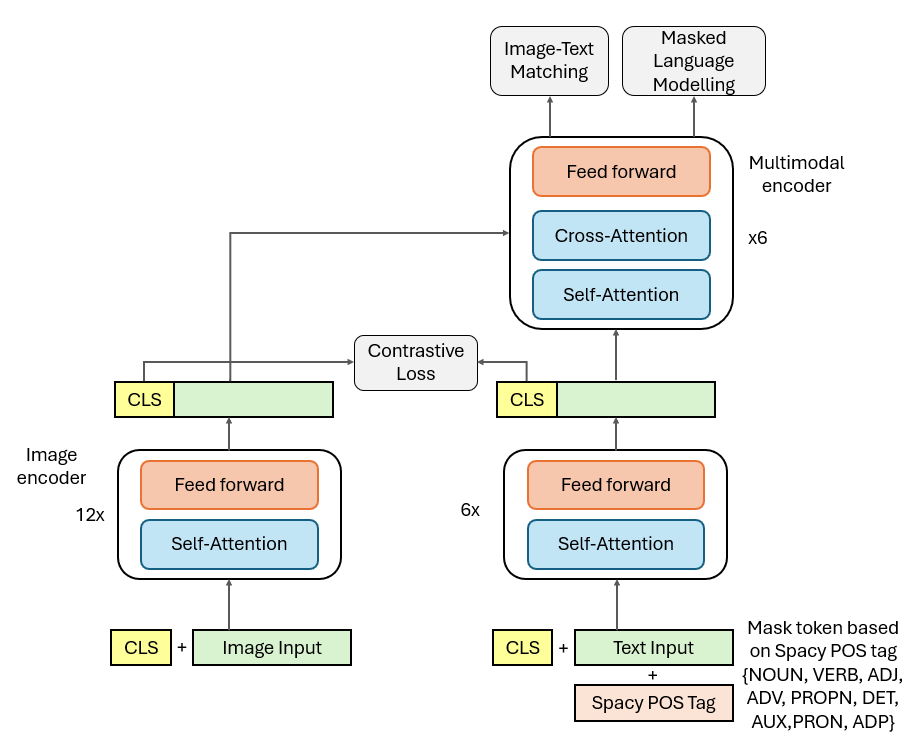
\includegraphics[width=0.6\textwidth]{Images/overview.png}
    \end{center}
    \small
\end{figure}

\section{Objective}
The objectives for our experiment are as listed.
\begin{enumerate}
    \item Develop a pre-trained \acrshort{vl} model to evaluate the impact of masking each \acrshort{pos} on performance and training dynamics.
    \item Benchmark the performance of our masking approach using specialized datasets \cite{valse, foil-dataset}, to gain a deeper understanding of masking effects.
    \item Analyze the effects of part-of-speech masking in the fine-tuning setup to understand its effect and performance in \acrshort{vl} task.
\end{enumerate}

\section{Scope}
\begin{enumerate}
    \item The training and testing datasets are both natural images.
    \item The model architecture is a cross-attention model, chosen for its ability to jointly predict answers based on information from multiple modalities.
    \item The fine-tuning dataset is in the same domain as the training dataset.
\end{enumerate}


